% cost_chain_flowchart.tex
% Standalone TikZ flowchart of the per-arrest cost chain modeled in
% estimate_costs.do. Compile with: pdflatex cost_chain_flowchart.tex
%
% Each stage box: stage name + per-incidence cost (incurred if reached).
% Each forward edge: transition probability to the next stage.
% Dashed edges: exits (dismissal / no-cost outcome / exoneration).
% Sentence cost is shown generalized -- per-class values come from the SPAC
% empirical lookup and trafficking statute (see sentence_lengths.do).

\documentclass[border=10pt]{standalone}
\usepackage{tikz}
\usepackage{amsmath, amssymb}
\usetikzlibrary{arrows.meta, positioning, shapes.geometric, calc, fit, backgrounds}

%% ============================================================
%% Probability parameters -- edit values here to update diagram.
%% These live in the preamble so this file compiles on its own
%% (pdflatex cost_chain_flowchart.tex). When this file is \input
%% into main.tex / methodology.tex via the standalone package,
%% this preamble is ignored and the host document's own copies of
%% these macros are used instead -- so there is no clash.
%% ============================================================
% Colorimetric (roadside) test
\newcommand{\pColorFP}{0.037}     % colorimetric false-positive rate
\newcommand{\pColorTN}{0.963}     % 1 - pColorFP (true neg. / false neg.)
% Handheld (station) confirmatory test -- only used "w/ law"
\newcommand{\pHandheldFP}{0.001}  % handheld FP rate (passes through to booking)
% Main chain transitions
\newcommand{\pBookFromArr}{1.00}  % Arrest -> Booking (w/o law scenario)
\newcommand{\pArrFromBook}{1.00}  % Booking -> Arraignment
\newcommand{\pPreFromArr}{1.00}   % Arraignment -> Pretrial
\newcommand{\pBrFromPre}{0.95}    % Pretrial -> Bail Review
\newcommand{\pPassBr}{0.95}       % Bail Review -> bond fork (1 - dismissed)
\newcommand{\pDisBr}{0.05}        % Dismissed at bail review
\newcommand{\pRel}{0.90}          % Released on recog.
\newcommand{\pHome}{0.05}         % Home confinement
\newcommand{\pHeld}{0.05}         % Held in custody
\newcommand{\pPrep}{1.00}         % Bond fork -> Case Prep
\newcommand{\pPres}{0.34}         % Case Prep -> Case Presentation
\newcommand{\pDisCp}{0.66}        % Charges dismissed at case prep
\newcommand{\pCoFromPres}{0.38}   % Case Presentation -> Costed Outcome
\newcommand{\pNoCost}{0.62}       % No-cost outcome
% Cumulative reach (per arrest, baseline / "w/o law" scenario)
\newcommand{\PArrest}{1.000}
\newcommand{\PBook}{1.000}
\newcommand{\PArr}{1.000}
\newcommand{\PPre}{0.950}
\newcommand{\PBr}{0.950}
\newcommand{\PCp}{0.903}
\newcommand{\PCpres}{0.307}
\newcommand{\PCo}{0.117}

\begin{document}

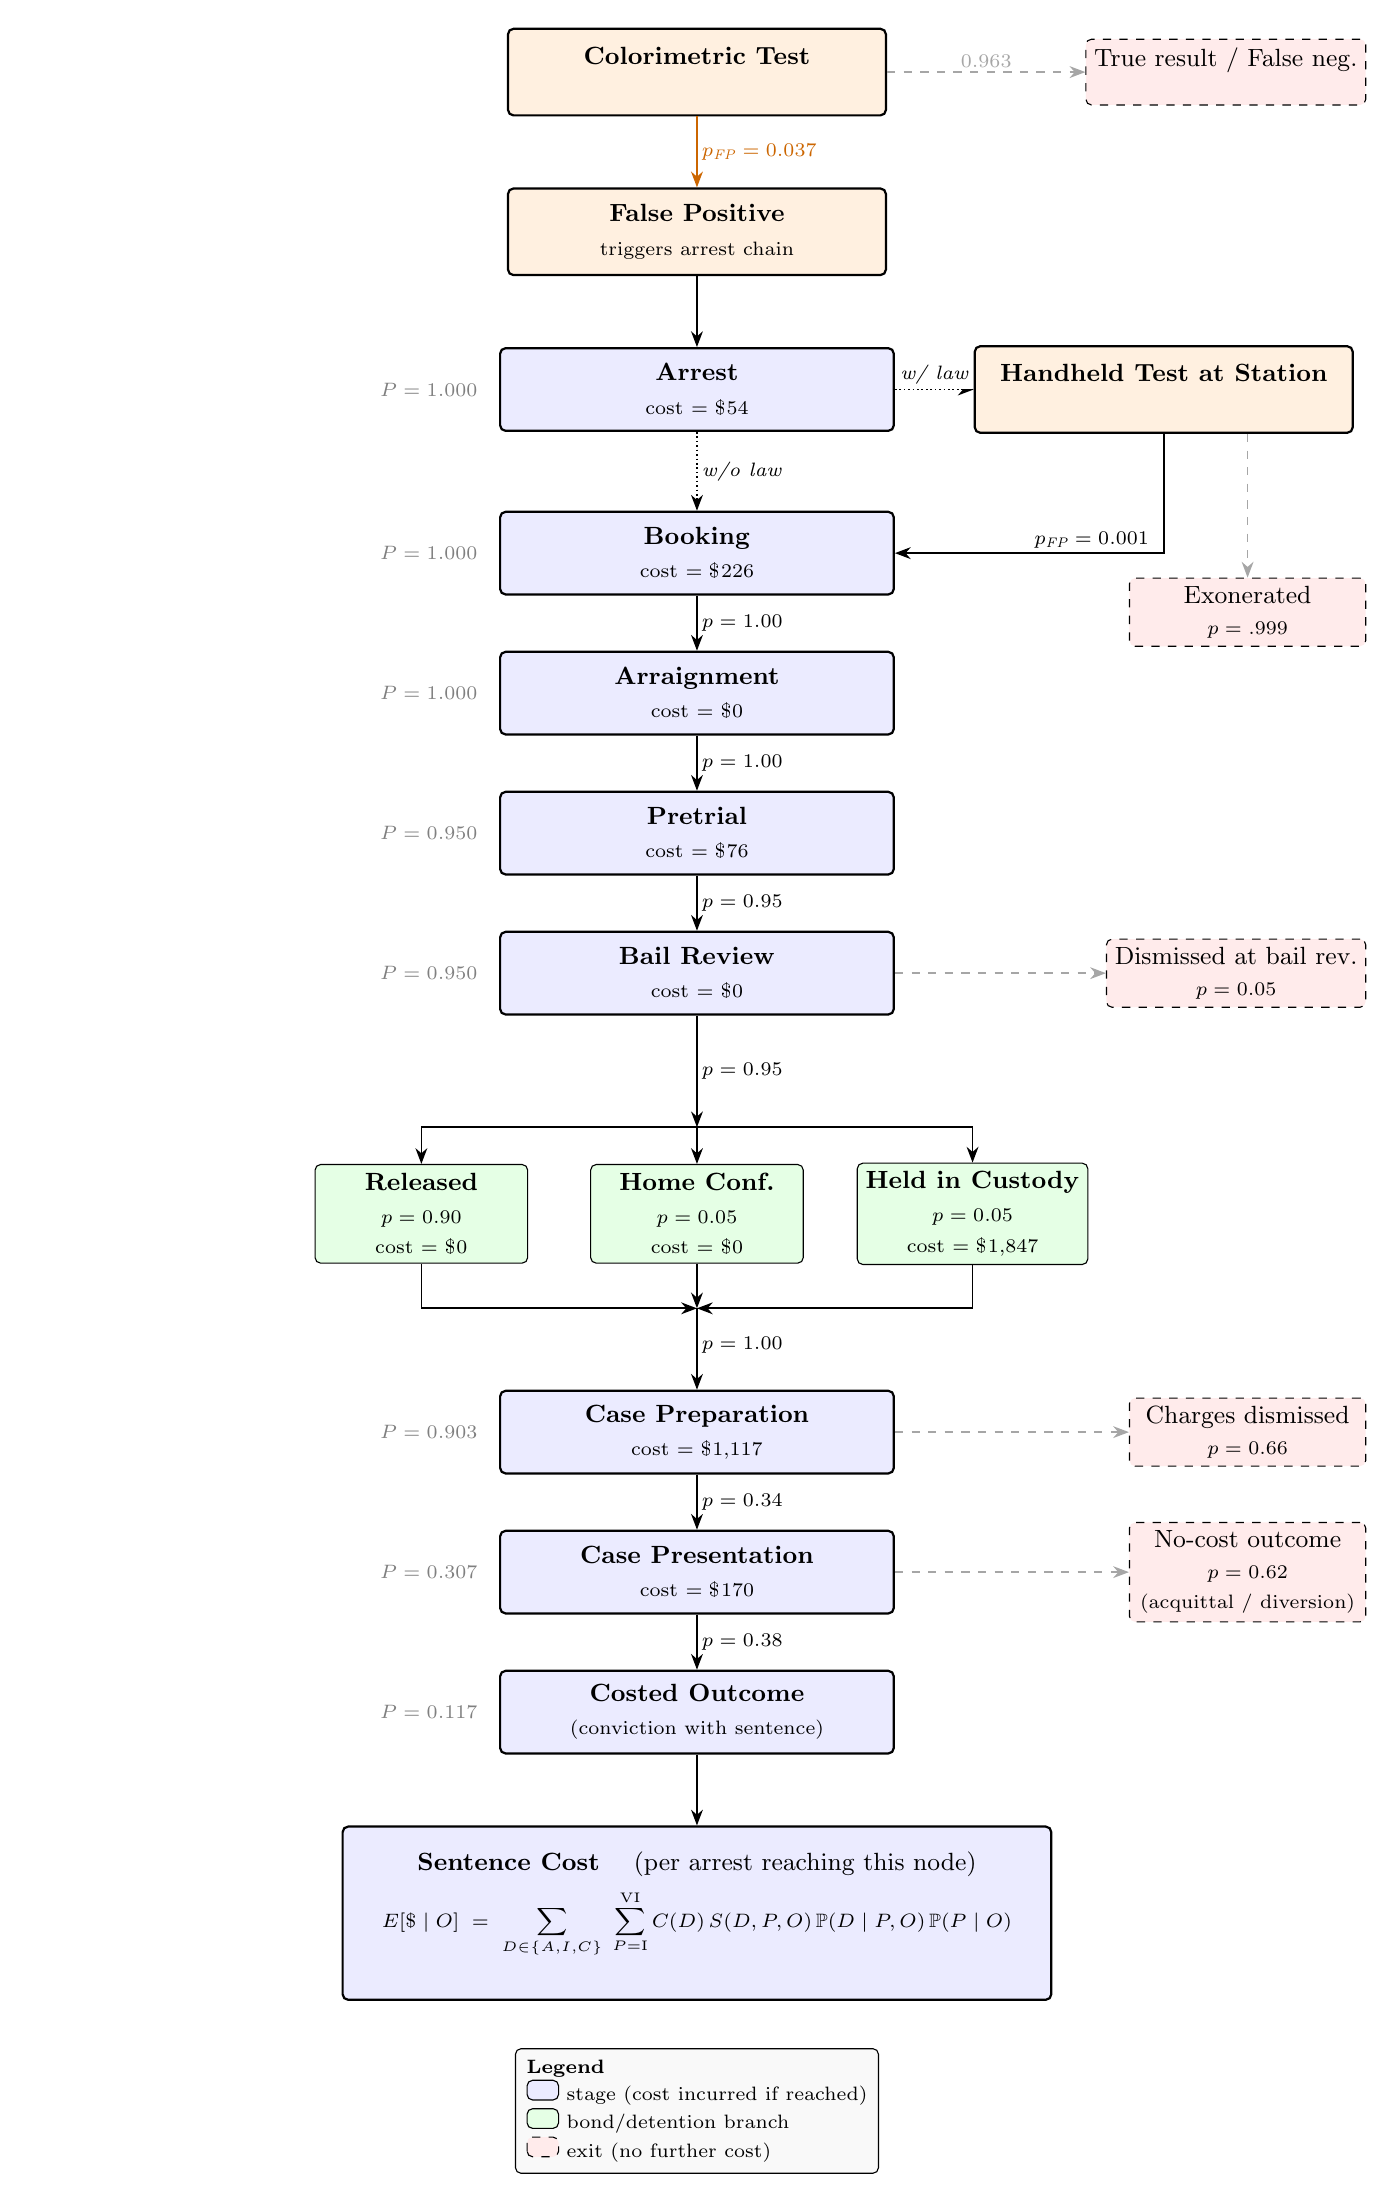
\begin{tikzpicture}[
  every node/.style = {font=\small, align=center},
  stage/.style    = {rectangle, draw, rounded corners=2pt, fill=blue!8,
                     thick, minimum width=5cm, minimum height=1.05cm,
                     inner sep=4pt},
  bond/.style     = {rectangle, draw, rounded corners=2pt, fill=green!10,
                     minimum width=2.7cm, minimum height=1.1cm, inner sep=3pt},
  exit/.style     = {rectangle, draw, rounded corners=2pt, fill=red!8,
                     dashed, minimum width=3cm, minimum height=0.8cm,
                     inner sep=3pt},
  sentence/.style = {rectangle, draw, rounded corners=2pt, fill=blue!8,
                     thick, minimum width=9cm, minimum height=2.2cm,
                     inner sep=6pt},
  colortest/.style= {rectangle, draw, rounded corners=2pt, fill=orange!12,
                     thick, minimum width=4.8cm, minimum height=1.1cm,
                     inner sep=4pt},
  arr/.style      = {-Stealth, semithick},
  dotarr/.style   = {-Stealth, semithick, densely dotted},
  exitarr/.style  = {-Stealth, semithick, dashed, gray!70},
  elab/.style     = {font=\scriptsize\itshape, fill=white, inner sep=1.5pt}
]

%% -------- Pre-arrest colormetric stack (above Arrest) --------
\node[colortest]                       (cm) at (0, 4.2) {\textbf{Colorimetric Test}\\[1pt]
                                                          };
\node[colortest,
      below=0.9cm of cm]               (fp) {\textbf{False Positive}\\[1pt]
                                              \scriptsize triggers arrest chain};

%% -------- Main vertical chain --------
\node[stage, below=0.9cm of fp]  (a)  {\textbf{Arrest}\\[1pt]
                                        \scriptsize cost = \$54};
\node[stage, below=1.0cm of a]   (b)  {\textbf{Booking}\\[1pt]
                                        \scriptsize cost = \$226};
\node[stage, below=0.7cm of b]   (ar) {\textbf{Arraignment}\\[1pt]
                                        \scriptsize cost = \$0};
\node[stage, below=0.7cm of ar]  (pt) {\textbf{Pretrial}\\[1pt]
                                        \scriptsize cost = \$76};
\node[stage, below=0.7cm of pt]  (br) {\textbf{Bail Review}\\[1pt]
                                        \scriptsize cost = \$0};

%% -------- Handheld station test (right of Arrest) --------
\node[colortest, right=1.0cm of a]   (hh) {\textbf{Handheld Test at Station}\\[1pt]
                                            };
%% Shared right-edge coordinate -- every exit box is anchored east at this x,
%% so their right edges all line up regardless of internal width.
\coordinate (exitR) at (8.5, 0);
\node[exit, anchor=east] (tn)     at (exitR |- cm)    {True result / False neg.\\};
\node[exit, anchor=east] (exon)   at ($(exitR |- b) - (0,0.75)$)     {Exonerated\\ \scriptsize $p = .999$};

%% -------- Bond fork (3 parallel branches) --------
\node[bond] (rel)  at (-3.5, -10.3) {\textbf{Released}\\[1pt]
                                     \scriptsize $p=\pRel$\\ \scriptsize cost = \$0};
\node[bond] (home) at ( 0,   -10.3) {\textbf{Home Conf.}\\[1pt]
                                     \scriptsize $p=\pHome$\\ \scriptsize cost = \$0};
\node[bond] (held) at ( 3.5, -10.3) {\textbf{Held in Custody}\\[1pt]
                                     \scriptsize $p=\pHeld$\\ \scriptsize cost = \$1{,}847};

%% -------- Resume main column --------
\node[stage, below=1.6cm of home]  (cp)   {\textbf{Case Preparation}\\[1pt]
                                            \scriptsize cost = \$1{,}117};
\node[stage, below=0.7cm of cp]    (cpres){\textbf{Case Presentation}\\[1pt]
                                            \scriptsize cost = \$170};
\node[stage, below=0.7cm of cpres] (co)   {\textbf{Costed Outcome}\\[1pt]
                                            \scriptsize (conviction with sentence)};

%% -------- Generalized sentence cost --------
\node[sentence, below=0.9cm of co] (sent) {%
  \textbf{Sentence Cost} \quad (per arrest reaching this node) \\[4pt]
  \scriptsize $\displaystyle
    E[\$\mid O] \;=\;
        \sum_{D \in \{A,I,C\}} \;\sum_{P = \text{I}}^{\text{VI}}
        C(D)\,S(D, P, O)\,\mathbb{P}(D \mid P, O)\,\mathbb{P}(P \mid O)$ \\[5pt]
};

%% -------- Right-side exits (aligned vertically to their source stage) --------
\node[exit, anchor=east] (dis_br)  at (exitR |- br)    {Dismissed at bail rev.\\ \scriptsize $p=\pDisBr$};
\node[exit, anchor=east] (dis_cp)  at (exitR |- cp)    {Charges dismissed\\ \scriptsize $p=\pDisCp$};
\node[exit, anchor=east] (no_cost) at (exitR |- cpres) {No-cost outcome\\ \scriptsize $p=\pNoCost$\\ \scriptsize (acquittal / diversion)};

%% -------- Colormetric -> FP / TN edges --------
\draw[arr, orange!80!black] (cm) -- node[elab, right]{$p_{\text{FP}}=\pColorFP$} (fp);
\draw[exitarr] (cm) -- node[elab, above]{$\pColorTN$} (tn);
\draw[arr] (fp) -- (a);

%% -------- Arrest -> Booking fork (w/o law direct, w/ law via handheld) --------
\draw[dotarr] (a) -- node[elab, right]{w/o law} (b);
\draw[dotarr] (a) -- node[elab, above]{w/ law} (hh);
\draw[arr] (hh.south) |- node[elab, above right, pos=0.75]{$p_{\text{FP}}=\pHandheldFP$} (b.east);
\draw[exitarr] (hh.south -| exon) -- (exon);

%% -------- Forward arrows with prob labels --------
\draw[arr] (b)  -- node[elab, right]{$p=\pArrFromBook$} (ar);
\draw[arr] (ar) -- node[elab, right]{$p=\pPreFromArr$} (pt);
\draw[arr] (pt) -- node[elab, right]{$p=\pBrFromPre$} (br);

%% Bail review --> bond fork (with pPassBr = 1 - dismissed)
\coordinate (fork) at (0, -9.2);
\draw[arr] (br.south) -- node[elab, right]{$p=\pPassBr$} (fork);
\draw[arr] (fork) -| (rel.north);
\draw[arr] (fork) -- (home.north);
\draw[arr] (fork) -| (held.north);

%% Bond branches converge into Case Prep
\coordinate (merge) at (0, -11.5);
\draw[arr] (rel.south)  |- (merge);
\draw[arr] (home.south) -- (merge);
\draw[arr] (held.south) |- (merge);
\draw[arr] (merge) -- node[elab, right, pos=0.45]{$p=\pPrep$} (cp);

\draw[arr] (cp)    -- node[elab, right]{$p=\pPres$} (cpres);
\draw[arr] (cpres) -- node[elab, right]{$p=\pCoFromPres$} (co);
\draw[arr] (co)    -- (sent);

%% Dashed exits
\draw[exitarr] (br)    -- (dis_br);
\draw[exitarr] (cp)    -- (dis_cp);
\draw[exitarr] (cpres) -- (no_cost);

%% -------- Cumulative reach-probability annotations (left column) --------
\node[left=0.15cm of a,     font=\scriptsize\color{gray}] {$P=\PArrest$};
\node[left=0.15cm of b,     font=\scriptsize\color{gray}] {$P=\PBook$};
\node[left=0.15cm of ar,    font=\scriptsize\color{gray}] {$P=\PArr$};
\node[left=0.15cm of pt,    font=\scriptsize\color{gray}] {$P=\PPre$};
\node[left=0.15cm of br,    font=\scriptsize\color{gray}] {$P=\PBr$};
\node[left=0.15cm of cp,    font=\scriptsize\color{gray}] {$P=\PCp$};
\node[left=0.15cm of cpres, font=\scriptsize\color{gray}] {$P=\PCpres$};
\node[left=0.15cm of co,    font=\scriptsize\color{gray}] {$P=\PCo$};

%% -------- Legend --------
\node[draw, rounded corners=2pt, fill=gray!5, inner sep=4pt,
      below=0.6cm of sent.south,
      anchor=north, font=\scriptsize, align=left] (leg) {%
   \textbf{Legend} \\
   \tikz\draw[fill=blue!8]   (0,0) rectangle (0.4,0.25);\ stage (cost incurred if reached) \\
   \tikz\draw[fill=green!10] (0,0) rectangle (0.4,0.25);\ bond/detention branch \\
   \tikz\draw[fill=red!8, dashed] (0,0) rectangle (0.4,0.25);\ exit (no further cost)};

%% Symmetric left padding so the bounding box (and hence the figure) is
%% centered on the main vertical chain at x=0, mirroring the right-side
%% exits/handheld extent. Invisible -- only affects the bounding box.
\path (-8.5, 0);

\end{tikzpicture}

\end{document}
